\documentclass[12pt]{article}

\usepackage{graphicx}
\usepackage[style=authoryear]{biblatex}
\usepackage{setspace}
\addbibresource{references.bib}
\onehalfspacing

\begin{document}

\begin{titlepage}
	\centering
	
	%opening
	\title{Gamification of Gaussian Splats \\ {\large Rendering and animating multiple splats in a Unity scene}}
	
	\author{Bavo Verstraeten}
	
	
	
	\maketitle
\end{titlepage}
	
\begin{abstract}
Gaussian splatting has emerged as a powerful technique for real-time rendering of complex 3D scenes. While existing implementations focus on efficient rendering, their integration into interactive applications such as games remains underexplored. This thesis investigates the gamification of Gaussian splats in Unity, enabling multiple Gaussian splat GameObjects to coexist within a scene, each with its own transform and animation. A key challenge is ensuring correct rendering while maintaining real-time performance. A current popular approach, a widely used Unity extension, processes splats in a per-GameObject order rather than achieving a globally correct sorting of individual splats. This work aims to overcome these limitations by adapting its rendering pipeline.
\end{abstract}

\begin{titlepage}
\centering
\tableofcontents
\end{titlepage}
\section{Background}
\subsection{From Meshes to Gaussian Splatting}
\subsubsection{Triangle Meshes}
In the field of computer graphics, the efficient rendering of complex 3D scenes has consistently posed a significant challenge. Traditional rendering techniques predominantly rely on triangle meshes, where the representation of surfaces is approximated through a network of interconnected triangles. While these methods have proven effective in many applications, they encounter limitations when dealing with highly detailed or non-uniform data. Achieving photorealistic results in such cases necessitates considerable memory and computational resources. Furthermore, these approaches are heavily dependent on manually crafted 3D models, a process that is both time-consuming and requires skilled artist. The generation of models from video or a collection of images offers the potential for a significantly simpler and more scalable solution.
\begin{figure}[h!]
	\centering
	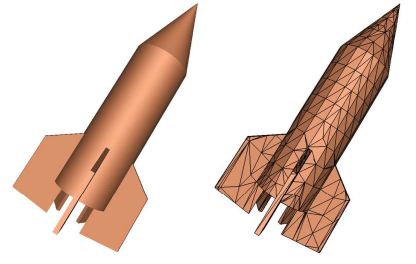
\includegraphics[width=\textwidth]{Images/TriangleMesh.png}
	\caption{Example of a triangle mesh, the most commonly used method for representing 3D objects in computer graphics. Image is taken from \cite{Mesh}}
	\label{fig:trianglemesh}
\end{figure}
\newpage
\subsubsection{Neural Radiance Fields}
One popular approach to addressing these challenges is Neural Radiance Fields (NeRF) \parencite{Nerf}, introduced in 2020. This method employs a neural network to learn a mapping from 3D position and viewing direction to an RGB color and density. The network is trained on a video or a collection of images, allowing it to reconstruct a scene by learning the underlying volumetric representation. During rendering, a ray is cast through each pixel of the screen, and multiple points along the ray are sampled. The neural network takes the position of each point and the viewing direction of the ray as input, producing color and density values. These outputs are then aggregated to compute the final color of the pixel, enabling the generation of photorealistic scenes without the need for manually crafted 3D models. However, due to the necessity of querying the neural network multiple times per pixel, this approach is computationally expensive and not suitable for real-time rendering.
\begin{figure}[h!]
	\centering
	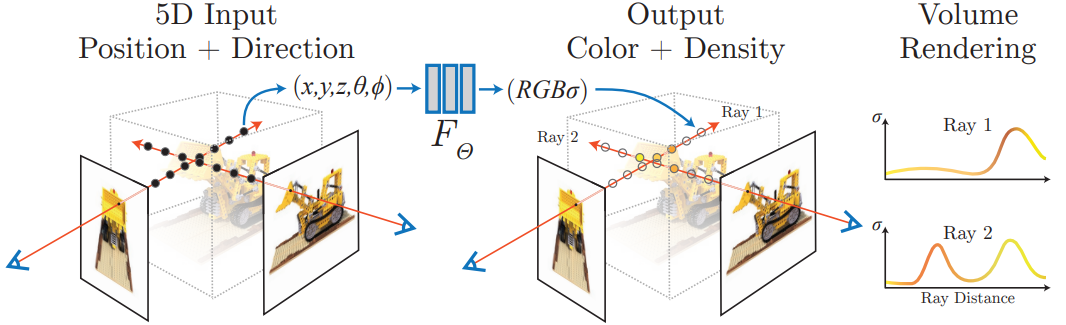
\includegraphics[width=\textwidth]{Images/Nerf.png}
	\caption{Rendering a scene using Neural Radiance Fields. Image is taken from \cite{Nerf}}
	\label{fig:nerf}
\end{figure}
\subsubsection{Gaussian Splatting}
In 2023, a method was introduced that retained the advantages of Neural Radiance Fields, while achieving real-time processing: Gaussian Splatting \parencite{OriginalSplatting}. Like Neural Radiance Fields, Gaussian Splatting uses a video or a collection of images as input to automatically generate the 3D scene data. However, rather than relying on a neural network to represent the data, the scene is represented as a collection of numerous small 3D Gaussians.
\begin{figure}[h!]
	\centering
	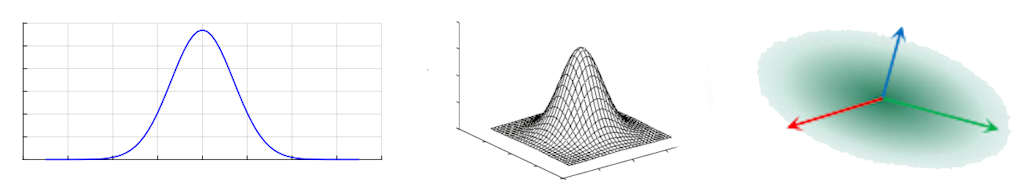
\includegraphics[width=\textwidth]{Images/GaussianForm.png}
	\caption{Illustration of Gaussian functions in different dimensions, shown left to right: 1D Gaussian \parencite{1DGaussian}, 2D Gaussian \parencite{2DGaussian}, and 3D Gaussian \parencite{3DGaussian}}
	\label{fig:Form}
\end{figure}
\newpage  \noindent
Each Gaussian is defined by several attributes that determine its appearance and behavior during rendering:
\begin{itemize}
	\item 3D coordinates
	\item Opacity (transparency)
	\item Anisotropic covariance: The degree to which the Gaussian is 'stretched' along each of the three axes independently
	\item Spherical Harmonics: The color of the Gaussian, which varies depending on the viewing angle
\end{itemize}
The key advantage of this approach is the way the scene is rendered. Instead of relying on rays or neural networks, which are computationally expensive, Gaussian Splatting leverages a rasterization technique. In this process, the 3D Gaussians are projected directly onto the 2D screen space, where they are rendered as small, disk-like splats. These splats are then blended together based on their spatial overlap, opacity, and color attributes.\\
Furthermore, state-of-the-art triangle mesh rendering also relies on rasterization, meaning that this approach already benefits from many well-established optimizations in graphics hardware. These optimizations, including efficient handling of spatial data and parallel processing, are directly applicable to Gaussian Splatting. By utilizing the same rendering pipeline, Gaussian Splatting can leverage these optimizations for further efficiency gains, making it an ideal choice for real-time rendering applications.
\subsection{Unity Extension Pipeline}
When it comes to the gamification of this technique, multiple engines come to mind, such as Unity, Godot, and Unreal Engine. Among these, Unity was chosen due to prior experience with the engine. Additionally, a widely referenced GitHub project \parencite{Aras} implementing Gaussian splatting in Unity provides a strong foundation for further research. This project stands out not only for its recognition within the community \parencite{ArasRecc1} \parencite{ArasRecc2}, but also for its developer, Aras Pranckevičius, a former Unity engineer with 15 years of experience working on the engine. His expertise suggests that the rendering pipeline adaptations are both well-optimized and efficiently integrated, making this implementation a suitable choice for exploration and development.
\\\\
Before examining the objectives of this thesis and the adaptations made to the selected implementation, it is essential to first outline the relevant aspects of its rendering pipeline. The discussion will focus solely on components that directly influence the rendering process. Certain aspects, such as the compression and storage of Gaussian splats in files, among others, fall outside the scope of this explanation and will not be covered.
\section{Experiments and Development}
\subsection{Preparing the scene}
\subsection{Initial Workarounds and Approximate Solutions}
\subsection{Towards a Correct Rendering Pipeline}

\addcontentsline{toc}{section}{References}
\printbibliography
\end{document}
